\chapter{Introducción}
\label{cap:capitulo1}
\setcounter{page}{1}

\begin{flushright}
\begin{minipage}[]{10cm}
\emph{El éxito es la suma de pequeños esfuerzos repetidos día tras día.}\\
\end{minipage}\\

Robert Collier\\
%Autor, \textit{Título}\\
\end{flushright}

\vspace{1cm}



%[Sección sobre la robótica y la importancia de la exploración espacial]
\section{La robótica}
\label{sec:robotica} % etiqueta para luego referenciar esta sección

%[Párrafo sobre la definicion de robótica y de robot]
La robótica es un campo multidisciplinario que se concentra en el diseño,
construcción, programación y operación de robots.
Estos dispositivos electromecánicos, con frecuencia modelados
antropomórficamente o zoomórficamente, están destinados a realizar tareas de
manera autónoma o semiautónoma en una variedad de entornos, para lo que disponen
de sensores que les proveen de información del medio que les rodea, de cierta
capacidad de cómputo para tomar decisiones acerca de estos datos recolectados, y
de actuadores que les permiten interactuar con el mismo y llevar a cabo dichas
decisiones.
Siendo así, sus capacidades y limitaciones están determinadas por su
\textit{hardware}, mientras que su inteligencia reside en su \textit{software}.
\\

%[Párrafo sobre la evolución de la robótica y su aplicación en nuestra sociedad]
Este gran campo de estudio e investigación ha experimentado un rápido
crecimiento y expansión desde sus inicios en la década de 1950, abarcando una
amplia gama de aplicaciones en la industria, la medicina, el entretenimiento y
la exploración espacial, entre muchas otras, y se encuentra en constante
evolución, desempeñando un papel cada vez más importante en nuestra sociedad
moderna, gracias en gran medida a los incesantes avances en tecnologías como la
inteligencia artificial, los sensores, los procesadores y los actuadores.



%[Sección sobre la importancia de la robótica en los avances científicos]
\section{La robótica en la ciencia}
\label{sec:exploracion_espacial} % etiqueta para luego referenciar esta sección

%[Párrafo sobre la importancia de la propia exploración espacial]
La robótica ha conformado un factor crucial en la exploración espacial, y esta
ha impulsado la creación de nuevas tecnologías que han sido desarrolladas
exclusivamente para ciertas misiones espaciales pero que luego se han aplicado
en la Tierra, mejorando la calidad de vida de las personas.
Ejemplos destacados incluyen los sistemas de purificación de agua, los tejidos
avanzados como la viscoelástica, los pañales y los dispositivos de imágenes
médicas, como la resonancia magnética, que han proporcionado a las personas
acceso a agua potable en regiones remotas, a colchones y almohadas que promueven
un mejor descanso, a mayores facilidades en cuanto al cuidado de los niños y
mayores, y a diagnósticos médicos precisos sin radiación nociva, lo cual ha
salvado innumerables vidas.
De esta manera, la investigación espacial no solo expande nuestro conocimiento
del universo, sino que también beneficia directamente a la humanidad en la
Tierra.
\\

%[Párrafo sobre el rover Perseverance y el helicóptero Ingenuity]
En cuanto al papel de la robótica en este campo, podemos destacar ejemplos como
los resistentes robots enviados a diferentes planetas y lunas del sistema solar
en busca de datos científicos.
Numerosas misiones científicas lo evidencian, como la misión \textit{Mars 2020}
de la NASA\footnote{
\href{https://science.nasa.gov/mission/mars-2020-perseverance/}{https://science.nasa.gov/mission/mars-2020-perseverance/}},
cuyos robots se ven ilustrados en la Figura \ref{fig:rover}, tomada por uno de
los robots, el rover Perseverance, que depositó con éxito al segundo robot sobre
la superficie marciana, el helicóptero Ingenuity, que aparece más al fondo en la
imagen, y que ayudó al rover a llevar a cabo su exploración y toma de muestras.
Este helicóptero estaba diseñado para realizar cinco vuelos durante un mes a
modo de demostrador tecnológico, pero su misión pudo alargarse hasta casi los
tres años, que cumplió el pasado 25 de Enero, momento en el que termina debido a
la rotura de una de sus palas, sumando entonces un total de 72 vuelos.

\begin{figure} [h!]
  \begin{center}
    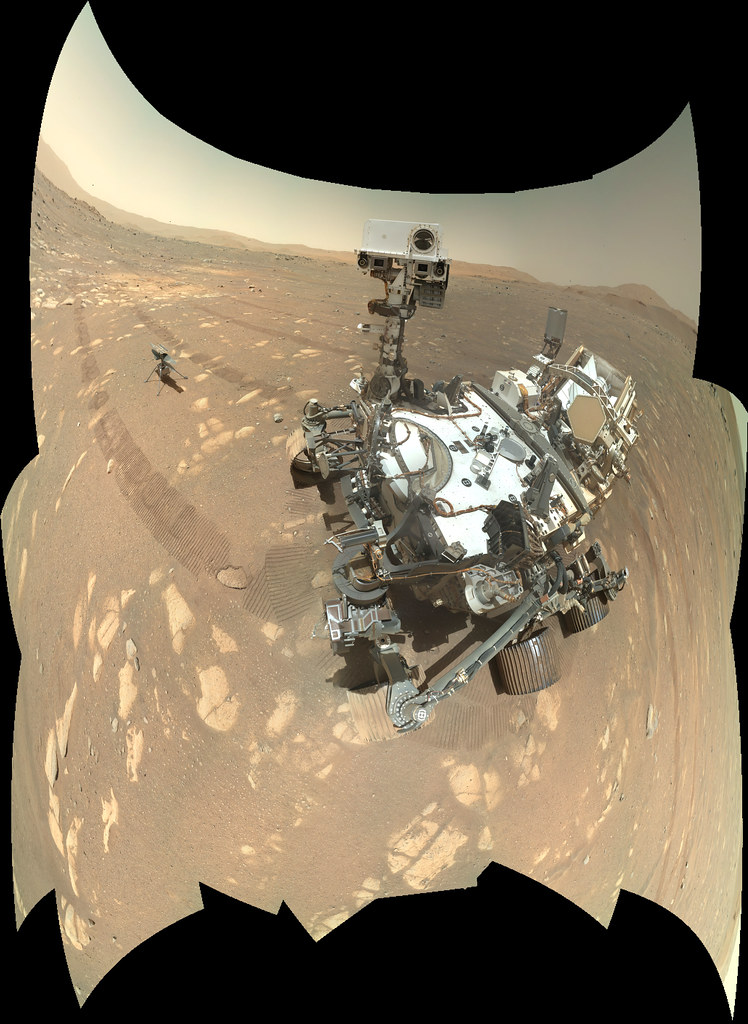
\includegraphics[width=8cm]{figs/perseverance_ingenuity_selfie_panorama}
  \end{center}
  \caption{Rover Perseverance e Ingenuity de la NASA en Marte \cite{perseverance_ingenuity}.}
  \label{fig:rover}
\end{figure}\

%[Párrafo de enlace con la robótica móvil]
Para el éxito de esta misión fue clave la investigación en múltiples ámbitos,
como la robótica móvil y todos los campos que esta conlleva, como pueden ser la
visión artificial, la navegación o la localización; áreas clave que no solo
están redefiniendo los límites de la tecnología, sino que también tienen un gran
impacto en cómo la utilizamos en nuestra vida diaria; como ha sucedido, por
ejemplo, con las aspiradoras robóticas o la conducción autónoma, que
inevitablemente ya forman parte de nuestra sociedad.



%[Sección sobre la robótica móvil y su relación con la educación]
\section{La robótica móvil}
\label{sec:robotica_movil} % etiqueta para luego referenciar esta sección

%[Párrafo sobre la robótica móvil]
La robótica móvil ha emergido como un campo multidisciplinario que fusiona la
ingeniería, la inteligencia artificial y múltiples ramas de la robótica y la
mecatrónica para crear sistemas capaces de moverse y operar en entornos
dinámicos, aprovechando áreas como la robótica de campo, la creación de mapas,
la localización y la navegación con ayuda de otros campos como la visión
artificial o la manipulación de objetos.
\\

Desde sus inicios, la robótica móvil ha sido impulsada por los avances
tecnológicos, permitiendo su aplicación en una amplia gama de entornos, desde la
exploración espacial y submarina, hasta la logística industrial y la atención
médica, siendo ya parte indispensable de nuestras vidas y mejorando la calidad
de las mismas.
En este contexto, la investigación en robótica móvil se centra en desarrollar
sistemas autónomos capaces de navegar de manera segura y eficiente en entornos
conocidos o desconocidos, adaptarse a cambios imprevistos y realizar tareas
complejas de manera autónoma.
\\

Un ejemplo representativo de este tipo de robots se puede ver en la Figura
\ref{fig:boston_dynamics}, donde se pueden observar dos de los robots más
desarrollados en el ámbito móvil, ambos de la empresa Boston Dynamics\footnote{
\href{https://bostondynamics.com/}{https://bostondynamics.com/}}, que han
demostrado una gran versatilidad en una variedad de entornos para ejecutar una
amplia variedad de tareas, desde abrir puertas, pasando por transportar cargas
de peso o realizar trabajos manuales, hasta incluso seguir rutinas deportivas
variadas, que en muchos casos iguala o incluso supera la de los humanos.

\begin{figure} [h!]
  \begin{center}
    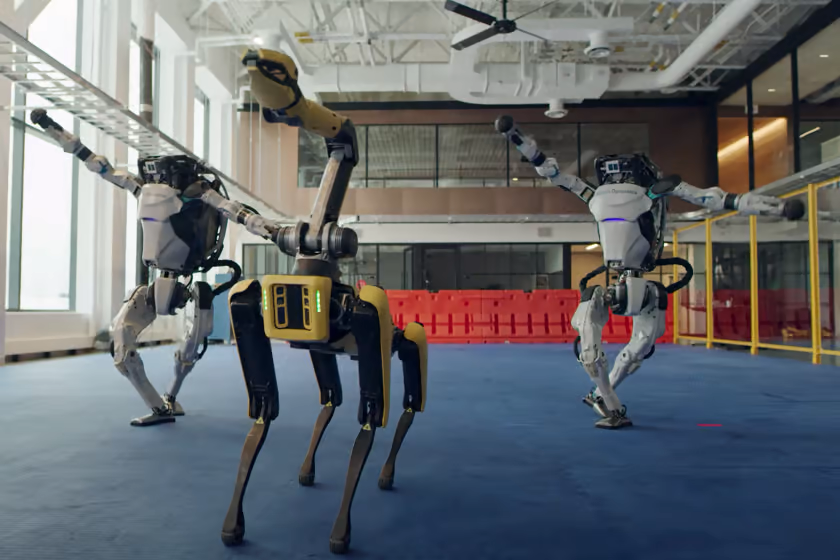
\includegraphics[width=8cm]{figs/atlas_spot_robots}
  \end{center}
  \caption{Robots Spot (frente) y Atlas (fondo) \cite{atlas_spot}.}
  \label{fig:boston_dynamics}
\end{figure}\

%[Párrafo introductorio a la localización]
En concreto, la autolocalización de los robots juega una papel importante en la
robótica móvil debido a la indispensable necesidad de conocer su ubicación
exacta a la hora de navegar por el entorno, que normalmente se consigue tomando
puntos de referencia gracias a los sensores y creando un modelo probabilístico
de la posición del robot basado en estos datos.
\\

%[Párrafo introductorio a la navegación]
Por su parte, para el correcto funcionamiento de la navegación, es indispensable
conocer la posición del robot durante el movimiento del mismo, para tener la
capacidad de sortear obstáculos y poder desplazar el robot al objetivo.
\\

%\cite{Trawny2009} %multilocalización probabilística cooperativa unidimensional,
%                  %filtro kalman.
%\cite{Fox2000}    %multilocalización probabilística basada en sensores y
%                  %balizas visuales.
%[Párrafo introductorio a la multirobótica y trabajos de localización]
La robótica móvil también forma parte de campos más grandes y complejos, e
incluso sienta las bases de algunos de ellos, como sucede con la multirobótica,
que representa un paso adelante en la complejidad y la escala de los sistemas
robóticos individuales, y permite realizar tareas que un solo robot no es capaz
de hacer, o realizarlas mucho mas rápidamente o eficientemente.
Como ejemplo de esta ventaja, son notables ciertos trabajos realizados sobre
localización con múltiples robots, como en el artículo \cite{Trawny2009}, en el
que se ponen a prueba las mismas técnicas utilizadas para un solo robot y
evalúan su viabilidad en un entorno unidimensional.
\\

También se han realizado trabajos enfocados a entornos tridimensionales, como se
observa en el artículo \cite{Fox2000}, en el cuál se logra una localización
basada en sensores, teniendo en cuenta la posición de los demás robots y
aumentando de este modo la precisión de la localización del propio robot en
cuestión.
\\

%[Párrafo sobre la educación en relación con la robótica móvil]
Además, este campo supone una gran oportunidad para el proceso de
enseñanza-aprendizaje, como se verá en la Sección \ref{sec:robotica_educativa},
ya que juega un papel crucial en el desarrollo de habilidades tecnológicas a la
vez que en la motivación de los estudiantes, los cuales obtienen una gran
sensación de realización y entusiasmo por aprender, al poder visualizar los
resultados en movimiento de manera autónoma.



%[Sección sobre la educación en robótica]
\section{La robótica educativa}
\label{sec:robotica_educativa} % etiqueta para luego referenciar esta sección

%[Párrafo sobre la demanda de educación en robótica en el mundo]
Debido a la creciente participación de los robots móviles en nuestras vidas
diarias, como se ha hecho notar en el caso de las aspiradoras robóticas, la
relevancia de la robótica en el ámbito educativo ha ido ganando terreno en los
últimos años, tanto en la comunidad europea como en otros muchos países.
Esto ha dado lugar a un aumento en la implementación de programas educativos las
cuales incluyen actividades prácticas de robótica en escuelas de educación
primaria y secundaria, promoviendo la creatividad, el pensamiento crítico y las
habilidades tecnológicas entre los estudiantes, además de fomentar el trabajo en
equipo y la resolución de problemas complejos, preparándolos de este modo para
futuros grados o carreras relacionadas con la tecnología, cuya demanda aumenta
año tras año.
\\

%[Párrafo sobre las competiciones robóticas educativas en España]
En el caso de España, desde la década de los 90, se han implementado programas
piloto y competiciones robóticas, como el programa Robolot\footnote{
\href{https://www.robolot.online/}{https://www.robolot.online/}} (1992),
desarrollado por la UPC, las Olimpiadas de Informática\footnote{
\href{https://olimpiada-informatica.org/}{https://olimpiada-informatica.org/}}
(1993), que incorporaron desafíos relacionados con la programación de robots,
así como la Robocampeones\footnote{
\href{https://tv.urjc.es/video/579f2bd5d68b1420378b50a2}{https://tv.urjc.es/video/579f2bd5d68b1420378b50a2}}
(1999), organizada en sus orígenes por la URJC y en la que cada año participan
más institutos o la competición RoboCupJunior\footnote{
\href{https://junior.robocup.org/}{https://junior.robocup.org/}} (2000),
ofreciendo a los estudiantes la oportunidad de diseñar, construir y programar
robots para competir en diferentes categorías.
\\

%[Párrafo sobre la educación en robótica en España]
Desde alrededor de 2014, dependiendo de la comunidad autónoma de España, se han
introducido programas y asignaturas que incluyen la robótica como parte esencial
del plan de estudios, en concreto en la Comunidad de Madrid, se implantaron
asignaturas relacionadas con la robótica en el itinerario formativo en la
educación entre 2014 y 2015.
Concretamente en la Educación Primaria en 2014, según el Decreto
\cite{Decreto2014}, se añadió la asignatura llamada \textit{Tecnología y
recursos digitales para la mejora del aprendizaje}, en cuyo anexo III se
describen los contenidos, que incluyen la programación en
\textit{Scratch}\footnote{
\href{https://scratch.mit.edu/}{https://scratch.mit.edu/}}.
Más tarde, en 2015, conforme al Decreto \cite{Decreto2015}, se añadió una
asignatura correspondiente al periodo de Educación Secundaria con el nombre
\textit{Tecnología, Programación y Robótica}, en cuyo anexo III se establecen
los contenidos, también basados en \textit{Scratch}, \textit{Arduino}\footnote{
\href{https://www.arduino.cc/}{https://www.arduino.cc/}} y la impresión 3D.
Toda esta información se puede ver resumida en el apartado 2.12 del artículo
\cite{EducacionRob}.
\\

%[Párrafo sobre las herramientas utilizadas en la educación en róbotica]
Al ser necesario un contexto simple y barato para la introducción de la
robótica, en educación se buscan herramientas como las placas \textit{Arduino}
(Figura \ref{fig:arduino}) o Raspberry Pi\footnote{
\href{https://www.raspberrypi.com/}{https://www.raspberrypi.com/}} (Figura
\ref{fig:raspberry_pi}), que presentan una amplia compatibilidad con distintos
sensores y actuadores y brinda un entorno sencillo para aquellos que se están
introduciendo en este campo y plataformas como \textit{Scratch} para simplificar
la programación gracias a su interfaz de bloques y la asociación de ideas a
colores, como se muestra en la Figura \ref{fig:scratch}.

\begin{figure}[h!]
  \centering
  \begin{minipage}{0.45\textwidth}
    \centering
    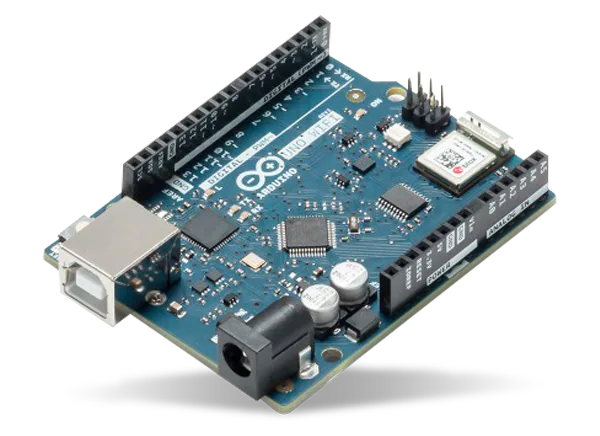
\includegraphics[width=7cm]{figs/arduino}
    \caption{Placa Arduino UNO \cite{arduino_uno}.}
    \label{fig:arduino}
  \end{minipage}
  \hfill
  \begin{minipage}{0.45\textwidth}
    \centering
    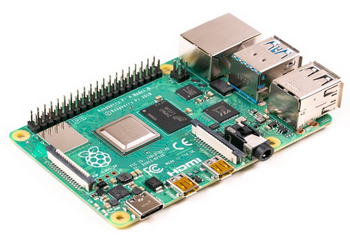
\includegraphics[width=7cm]{figs/raspberry_pi_4b}
    \caption{Raspberry Pi 4, modelo B \cite{raspberry_pi_4b}}
    \label{fig:raspberry_pi}
  \end{minipage}
\end{figure}\

%[Párrafo sobre la educación en relacion con la robótica móvil]
Las placas utilizadas en el ámbito educativo, mencionadas anteriormente,
resultan ideales para estos propósitos debido a su coste y simplicidad, sin
embargo, también imponen ciertas limitaciones en las capacidades del robot y en
la posibilidad de añadir \textit{hardware} externo más complejo y potente (sobre
todo en el caso de Arduino), como cámaras o LIDARs, siendo estos últimos
sensores dedicados a la medición de distancias mediante la emisión y recepción
de un láser, o actuadores como motores más potentes que a menudo requieren de
mayor alimentación eléctrica de la que estas placas pueden brindar.
Esto genera trabas a la propia originalidad y aprendizaje de los estudiantes,
restringiendo así su creatividad, innovación y potencial de creación, una vez se
han obtenido unos conocimientos básicos.

\begin{figure} [h!]
  \begin{center}
    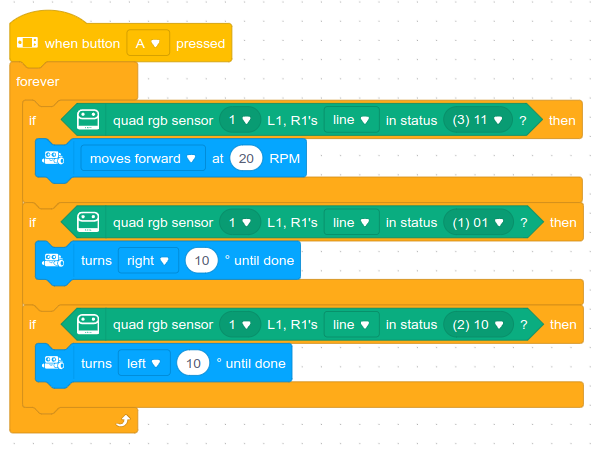
\includegraphics[width=8cm]{figs/scratch_arduino_code}
  \end{center}
  \caption{Código de Arduino en Scratch \cite{arduino_scratch_code}.}
  \label{fig:scratch}
\end{figure}\

%[Párrafo sobre el escalón de aprendizaje en la educación en robótica]
Para paliar las limitaciones de lenguajes básicos de programación como Scratch,
existe ROS \cite{ros}, cuyas siglas significan, en inglés, sistema operativo
de robots, aunque nada tiene que ver con ningún sistema operativo, siendo por el
contrario el \textit{middleware} estándar por excelencia en robótica, encargado
de abstraer del hardware al programador, y permitiéndolo, por tanto, un
desarrollo más ameno y compatible con una amplia gama de robots, cuya
arquitectura interna puede verse apreciada en la Figura \ref{fig:ros}, en la que
se ve comparada con la de su sucesor o versión posterior, ROS2 \cite{ros2}.
\\

Este proceso implica un considerable escalón de aprendizaje, ya que no solo se
debe dominar un lenguaje de programación más complejo, sino que también se debe
comprender el entorno que rodea a esta plataforma, en el que se incluyen campos
de la robótica como son las comunicaciones, la arquitectura \textit{software},
la programación modular y orientada a objetos, algoritmos y estructuras de
datos, entre otros muchos, y que suelen conllevar decenas de asignaturas con
identidad propia en cualquier grado universitario.
La teoría de la existencia de una brecha educativa en este ámbito se ve
respaldada por trabajos como la tesis doctoral de \cite{vega2018}, en cuyas
secciones A.3 y A.4, se analiza esta misma perspectiva y se propone una solución
respectivamente.

\begin{figure} [h!]
  \begin{center}
    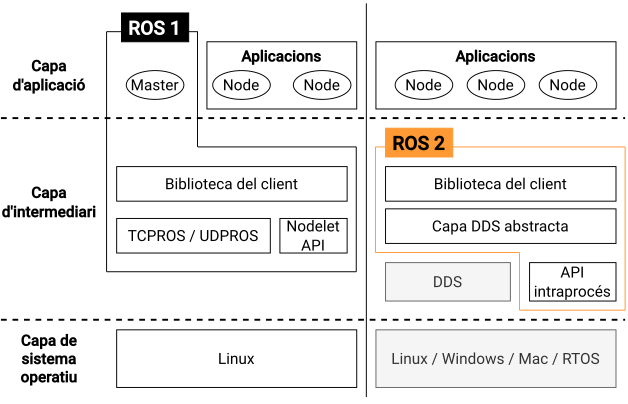
\includegraphics[width=12cm]{figs/ROS_and_ROS2}
  \end{center}
  \caption{Arquitecturas de ROS y ROS2 \cite{ros_ros2}.}
  \label{fig:ros}
\end{figure}\

%[Párrafo sobre la solución al escalón de aprendizaje en robótica]
Por este motivo, resulta evidente la necesidad de un paso intermedio que pueda
actuar como puente entre estos dos niveles de aprendizaje, el cual podría ser
incorporado, por ejemplo, en el programa educativo de la etapa de Educación
Secundaria o Bachillerato.
Este nivel intermedio facilitaría la transición entre esta etapa educativa y la
universitaria, concretamente dentro del ámbito científico-tecnológico.



%[Sección sobre la robótica de bajo coste]
\section{La robótica de bajo coste}
\label{sec:robotica_bajo_coste} % etiqueta para luego referenciar esta sección

%[Párrafo sobre la robótica de bajo coste]
La robótica de bajo coste se refiere al desarrollo e implementación de sistemas
robóticos, como los descritos anteriormente, utilizando componentes y recursos
económicos, con el objetivo de hacer la tecnología robótica más accesible y
asequible para una amplia gama de aplicaciones y usuarios.
Este enfoque busca reducir los costes asociados con la construcción y operación
de robots, empleando materiales económicos, hardware de bajo coste y técnicas
de fabricación eficientes.
\\

%[Párrafo sobre la robótica de bajo coste en relación con la robótica móvil]
En el contexto de la robótica móvil, los sistemas de bajo coste pueden ofrecer
soluciones viables para aplicaciones con presupuestos limitados o despliegues a
gran escala, abarcando un papel crucial en áreas como la educación, la
investigación académica, la asistencia social y la exploración de entornos
remotos o peligrosos.
Además de su utilidad práctica, la robótica de bajo coste también promueve la
innovación y el desarrollo de nuevas tecnologías al proporcionar una plataforma
accesible para la experimentación y la creatividad abierta a una amplia
comunidad.
\\

%[Párrafo ejemplificativo sobre la robótica de bajo coste]
Un ejemplo destacado de este tipo de robótica es el robot Sora-Q\footnote{
\href{https://www.takaratomy.co.jp/english/products/sora-q/}{https://www.takaratomy.co.jp/english/products/sora-q/}},
enviado a la Luna recientemente por la JAXA\footnote{
\href{https://global.jaxa.jp/}{https://global.jaxa.jp/}} y desarrollado por la
juguetería japonesa Takara Tomy\footnote{
\href{https://www.takaratomy.co.jp/english/}{https://www.takaratomy.co.jp/english/}},
que se mueve por la superficie lunar arrastrándose al rotar sus dos piezas
semiesféricas, lo que le da el aspecto y tamaño de una bola de béisbol.
Dicho robot, tras completar su misión, fue comercializado por 150\euro, hito que
ilustra cómo la tecnología robótica puede volverse accesible para un público más
amplio, incluso después de su participación en misiones espaciales.
\\

%[Párrafo sobre la robótica de bajo coste en relación con la educación]
De entre las distintas áreas en que se aplica este enfoque, cabe destacar la
robótica educativa, que suele basarse en este tipo de sistemas de bajo coste, ya
que las instituciones educativas enfrentan limitaciones presupuestarias que
dificultan la adquisición de sistemas más costosos, por el presupuesto limitado
y por el gran número de alumnos, a los que no podrían proveer de sistemas de
este calibre de otra manera; o no al menos de forma individual.
\\

%[Párrafo sobre los beneficios de la robótica de bajo coste en la educación]
La robótica de bajo coste no solo ha democratizado el acceso a la tecnología
robótica, sino que también ha revolucionado la forma en que se enseña la
robótica en las escuelas.
Este enfoque económico ha permitido a las instituciones educativas superar las
limitaciones presupuestarias y proporcionar a un mayor número de estudiantes la
oportunidad de involucrarse en actividades prácticas de robótica, allanando el
camino para que los estudiantes se sumerjan en áreas más avanzadas de este área,
como pueden ser la robótica móvil o campos estrechamente relacionados.



%[Sección sobre la robótica colaborativa / multirobótica]
\section{La robótica colaborativa}
\label{sec:robotica_colaborativa} % etiqueta para luego referenciar esta sección

%\cite{Verma2021}      %Resumen de multirobotica en general.
%\cite{Parker2003}     %Subcampos de multirobotica explicados (comunicación, la
%                      %planificación de tareas, la localización, la creación de
%                      %mapas, la manipulación de objetos, la coordinación de
%                      %robots, o robótica reconfigurable...).
%\cite{Sheng2006}      %Enfocado a descentralizacion, coordinacion y
%                      %optimizacion.
%\cite{Alami1998}      %Cooperacion, menor centralizacion, programar cada robot.
%\cite{Chaimowicz2001} %Coordinacion centralizada, los robots tienen la
%                      %capacidad de cambiar de rol.

%[Párrafo introductorio sobre la multirobótica]
La multirobótica es un campo de investigación que estudia y desarrolla sistemas
robóticos compuestos por múltiples robots que trabajan en conjunto para realizar
una amplia variedad de tareas complejas, y que ha sido ampliamente estudiada en
artículos como \cite{Verma2021}, en los que se relatan todos los aspectos de la
misma, poniendo en contexto este novedoso campo.
\\

%[Párrafo más específico sobre las tareas más relevantes en la multirobótica]
Estos sistemas pueden dividir sus tareas, como son la exploración de entornos
desconocidos o la búsqueda y rescate en áreas de difícil acceso, por lo que la
colaboración entre ellos es de vital importancia, e implica aspectos como el
establecimiento de comunicaciones para compartir información entre ellos y
entender de un mejor modo el mundo y contexto que les rodea, la creación de
mapas del entorno para poder localizarse y navegar por el mismo de manera
controlada o la manipulación de objetos, muchas veces necesaria para completar
el objetivo propuesto para estos sistemas.
Todo ello puede verse descrito en el trabajo de \cite{Parker2003}, en el que se
relatan con más detalle los avances logrados en estos aspectos.
\\

%[Párrafo sobre la importancia de la coordinación en la multirobótica]
La coordinación entre estos sistemas puede suponer la diferencia entre el éxito
o el fracaso de su misión, por lo que también es de suma importancia, y por ello
se han realizado múltiples trabajos acerca de este tema.
En estos términos, los equipos de robots pueden operar eficientemente asignando
roles y responsabilidades como expone el artículo \cite{Alami1998}, en el que se
desarrolla un sistema de control con la menor centralización posible para
estudiar la cooperación multirobot en el proyecto
MARTHA\footnote{MARTHA: European ESPRIT III Project No 6668 ``Multiple
Autonomous Robots for Transport and Handling Applications''}.
\\

%[Párrafo sobre la descentralización en la multirobótica]
A pesar de intentar crear sistemas con la mayor descentralización posible, el
trabajo anterior sigue siendo un sistema centralizado, donde un robot puede
asumir roles específicos.
La tendencia actual se inclina hacia sistemas directamente o casi totalmente
descentralizados, donde la coordinación y la optimización son fundamentales,
como se hace notar en el trabajo de \cite{Sheng2006}, en el que todos los robots
actualizan su propio mapa local con la información de los demás, sin que ninguno
de ellos adquiera un mayor protagonismo o importancia.
\\

Gracias a este tipo de trabajos, se ha conseguido mejorar la eficiencia y la
robustez de los sistemas robóticos, y la multirobótica se ha convertido en un
campo importante de investigación.
Los principios y problemas técnicos en este campo se exploran en diversos
contextos, como se ilustra en la Figura \ref{fig:multirobots}, en la cual, la
flota de robots está realizando pruebas de localización y navegación conjunta,
actualizando sus mapas utilizando la información de todos los robots.

\begin{figure} [h!]
  \begin{center}
    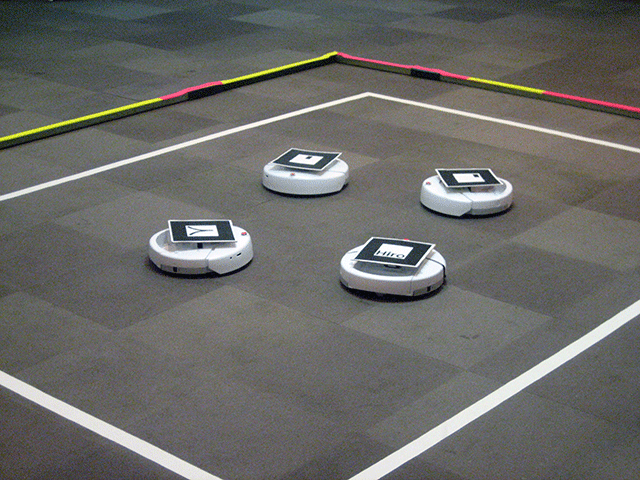
\includegraphics[width=8cm]{figs/multirobotics_navigation}
  \end{center}
  \caption{Múltiples robots navegando en conjunto \cite{multirobot_navigation}.}
  \label{fig:multirobots}
\end{figure}\

%[Párrafo sobre la multirobótica en educación].
En el ámbito educativo, la multirobótica ofrece una oportunidad única para
involucrar a los estudiantes en actividades prácticas y colaborativas.
Al trabajar con sistemas multirobot, los estudiantes no solo adquieren
conocimientos sobre programación, control y mecánica de robots, sino que también
exploran conceptos como son las telecomunicaciones entre robots, la coordinación,
la planificación y asignación de tareas con o sin prioridades, la localización y
navegación conjunta, como se ha explicado en los trabajos citados en la Sección
\ref{sec:robotica_movil}, así como la seguridad que se requiere para evitar
colisiones entre ellos, adquiriendo a su vez habilidades útiles para el trabajo
en equipo.
Además, este campo proporciona un entorno de aprendizaje dinámico y estimulante
que despierta aún más la curiosidad y la creatividad de los estudiantes,
preparándolos para enfrentar los desafíos del mundo tecnológico en constante
evolución.
\\

%[Párrafo sobre ejemplos de múltiples robots educativos].
Un ejemplo representativo de los robots educativos, en este caso del Laboratorio
de Robótica de la Universidad Rey Juan Carlos, aparece en la Figura
\ref{fig:robots_education}, en la que se pueden diferenciar dos modelos
distintos de robots: Turtlebot 2, en la parte superior de la imagen; y Turtlebot
4, más modernos, en la parte inferior de la misma.

\begin{figure} [h!]
  \begin{center}
    \includegraphics[width=8cm]{figs/multirobotics_education}
  \end{center}
  \caption{Robots educativos Turtlebot 2 (arriba) y Turtlebot 4 (abajo).}
  \label{fig:robots_education}
\end{figure}\



%[Sección sobre los flujos de datos en robótica]
\section{Flujos de datos en robótica}
\label{sec:flujos_datos} % etiqueta para luego referenciar esta sección

%[Párrafo sobre las telecomunicaciones entre robots]
Las mencionadas telecomunicaciones entre robots son fundamentales en la
multirobótica, ya que garantizan una comunicación rápida, óptima, eficiente y
ordenada entre los distintos dispositivos, necesaria para un correcto desempeño
de la funcionalidad en cuestión.
Sin embargo, este proceso puede enfrentarse a desafíos, como la congestión de la
red, y la consecuente pérdida de mensajes, que pueden ser críticos para el
correcto funcionamiento de los robots.
Por este motivo, resulta crucial gestionar cuidadosamente la cantidad de robots
y mensajes generados, intentando minimizarlos para optimizar el rendimiento del
sistema y evitando de esta manera el problema conocido como \textit{cuello de
botella}, siendo este el objetivo principal del estudio de los flujos de datos
en Robótica.
\\

%[Párrafo sobre flujos de datos y comportamiento reactivo mas simple para educación]
Un flujo de datos consiste en un grafo dirigido de los datos que fluyen entre
operaciones.
Mantener un flujo de datos correcto es fundamental para solventar los problemas
de telecomunicaciones mencionados en el desarrollo de sistemas de multirobótica.
Además, simplifica el desarrollo del software al proporcionar una clara visión
de la dirección, el sentido, el origen y el destino de los datos en cada
momento.
Esto permite dividir el programa en partes claramente diferenciadas, normalmente
llamadas nodos, modularizándolo y dando lugar a la división del problema último
en varios problemas más simples y fáciles de atajar, creando un paradigma que
modela el programa como un flujo de datos.
Como resultado, el desarrollo se vuelve un proceso más sostenible y escalable, y
por tanto, más fácil de llevar a cabo por los estudiantes.
\\

Este proceso se puede ver ilustrado en la Figura \ref{fig:data_flow_qr_example},
donde se ilustra, de manera simplificada, el flujo de datos de un robot
programado para detectar y seguir códigos QR\footnote{
\href{https://github.com/USanz/follow_beacon}{https://github.com/USanz/follow\_beacon}},
en la que se puede observar cómo los datos siguen un esquema de nodos dirigido,
en este caso unidireccional, pasando de su origen en el robot a su procesamiento
en otra máquina y acabando en su posterior vuelta al robot en forma de órdenes
de movimiento, pudiendo saber en todo momento en qué proceso se encuentran
dichos datos.

\begin{figure} [h!]
  \begin{center}
    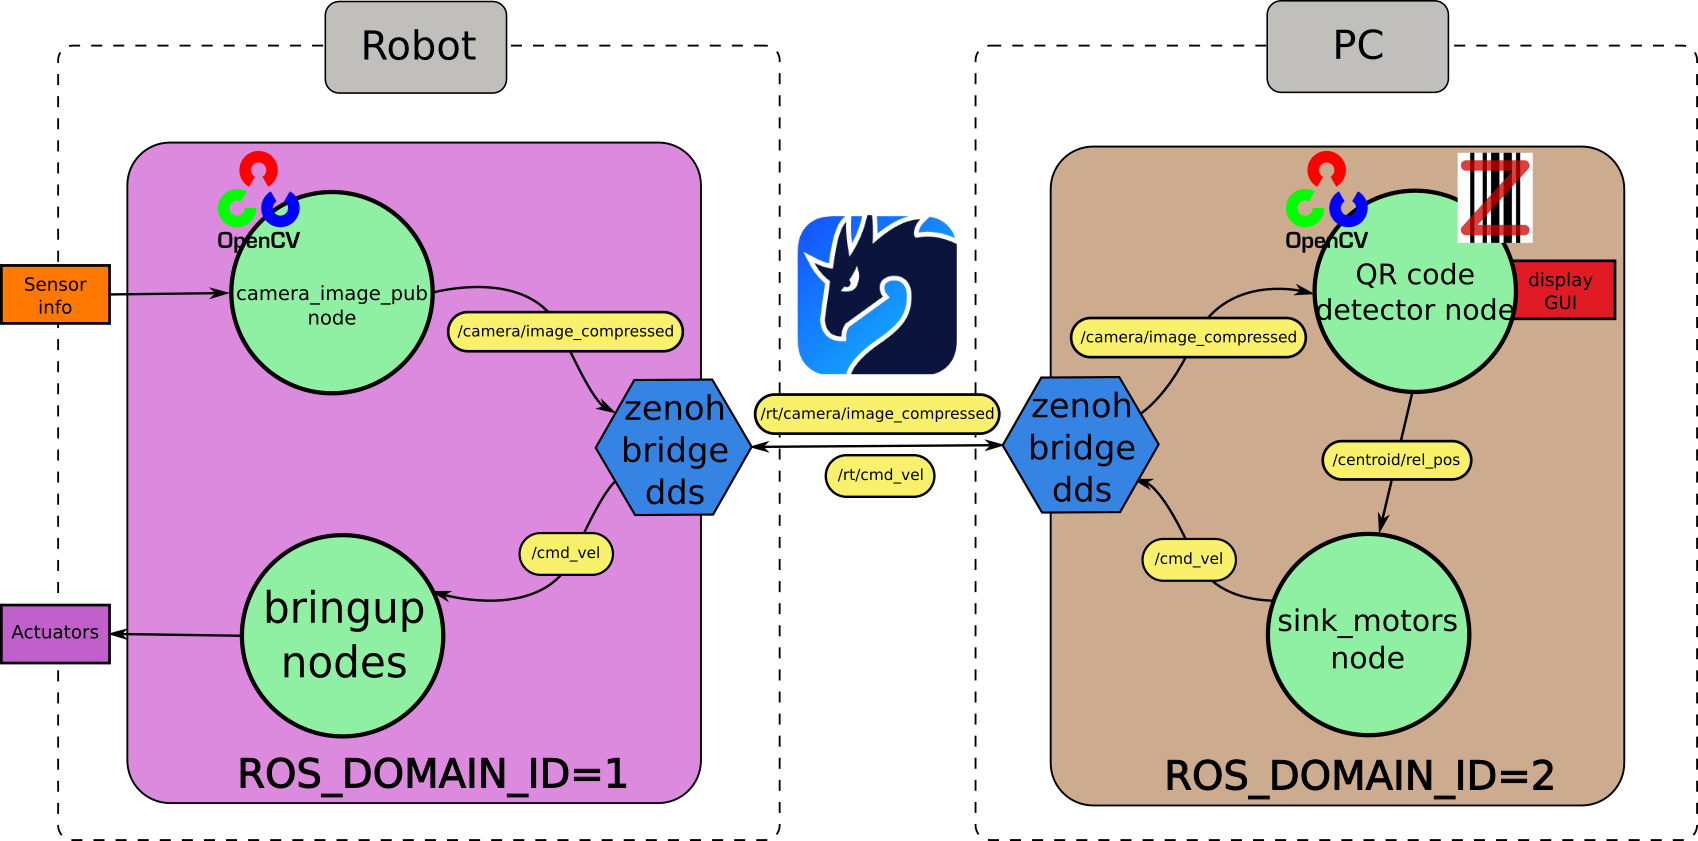
\includegraphics[width=15cm]{figs/QR_code_data_flow}
  \end{center}
  \caption{Flujo de datos de un robot para seguir códigos QR.}
  \label{fig:data_flow_qr_example}
\end{figure}\

Este proceso es equiparable a la forma de programación de un robot reactivo, ya
que, como se observa en la Figura \ref{fig:data_flow_vs_robotics}, en los flujos
de datos existen tres tipos esenciales de nodos: unos, en los que se originan
los datos; otros, donde se computan; y otros, donde los datos llegan a su final
y que encuentran correspondencia en los nodos encargados de la percepción de un
robot, del cómputo de estos datos obtenidos y de los nodos encargados de la
actuación del robot, respectivamente\footnote{
\href{https://www.youtube.com/watch?v=ZgFHCvEFU0I}{[Ponencia conf. ROSCON Madrid
2023] https://www.youtube.com/watch?v=ZgFHCvEFU0I}}.
Además, este tipo de programación de los robots de manera reactiva es el más
simple y el primero que se suele aprender, por lo que genera una sinergia con el
área educativa en este ámbito.

\begin{figure} [h!]
  \begin{center}
    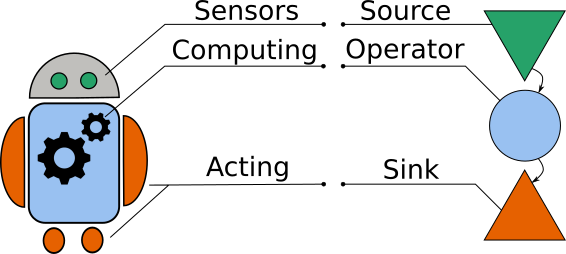
\includegraphics[width=9cm]{figs/data-flow_vs_robotics_scheme}
  \end{center}
  \caption{Comparación entre flujo de datos y diseño de robot.}
  \label{fig:data_flow_vs_robotics}
\end{figure}\


%Y, para terminar este capítulo, resume brevemente qué vas a contar en los siguientes.

El próximo capítulo detalla los objetivos planteados y logrados en este trabajo,
ofreciendo una perspectiva más completa de su finalidad.
